%% ------------------------------------------------------------------------- %%
\chapter{Fundamentação Teórica}
\label{cap:fundamentacao}

As primeiras televisões surgiram na decáda de XX do século passado \cite{WikipediaTelevisao}. Apartir desta descoberta, muito se evoluiu com relação as telas possibilitando ao consumirdor final mais qualidade com telas mais finas, imagens cada vez mais nítidas e brilhosas, além de outros atributos que são considerados para determinar a qualidade em telas.\\

Nos últimos anos surgiram diversas tecnologias de telas, veremos neste capítulo algumas informações das principais e últimas tecnologias utilizadas.

%% ------------------------------------------------------------------------- %%
\section{Plasma}
\label{sec:plasma}

\begin{figure}[!ht]
  \centering
  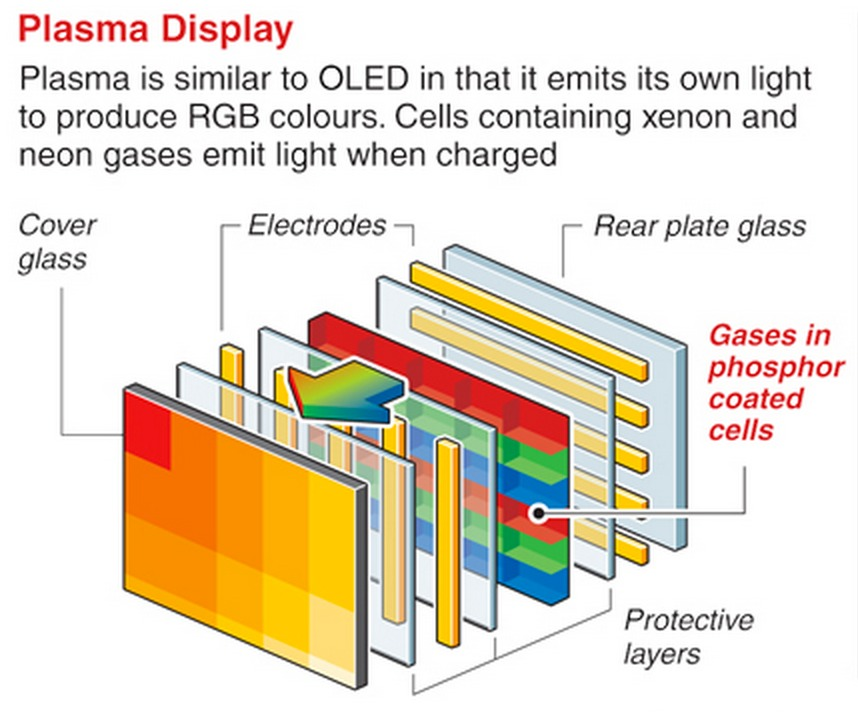
\includegraphics[width=.40\textwidth]{./figuras/camadas_plasma} 
  \caption{Camadas de uma Tela de Plasma}
  \label{fig:camadas_plasma} 
\end{figure}

Uma tela de plasma (português brasileiro) ou ecrã a plasma (português europeu) é um dispositivo baseado na tecnologia de painéis de plasma (PDP, Plasma Display Panel), que foi aprimorada na última década para o mercado da televisão de alta definição (HDTV). O funcionamento baseia-se na ionização de gases nobres (plasma) contidos em minúsculas células revestidas por fósforo.\\

Televisores de plasma têm tela totalmente plana e estão disponíveis em tamanhos até 150 polegadas, com resoluções até 2000 pixels. Apresentam excepcional reprodução de cores e são fabricados na proporção \textit{widescreen}. São painéis finos, de volume bastante reduzido em comparação aos monitores de tubo e retroprojeção com área de tela equivalente \cite{WikipediaTelaPlasma}. \\

\begin{figure}[!ht]
  \centering
  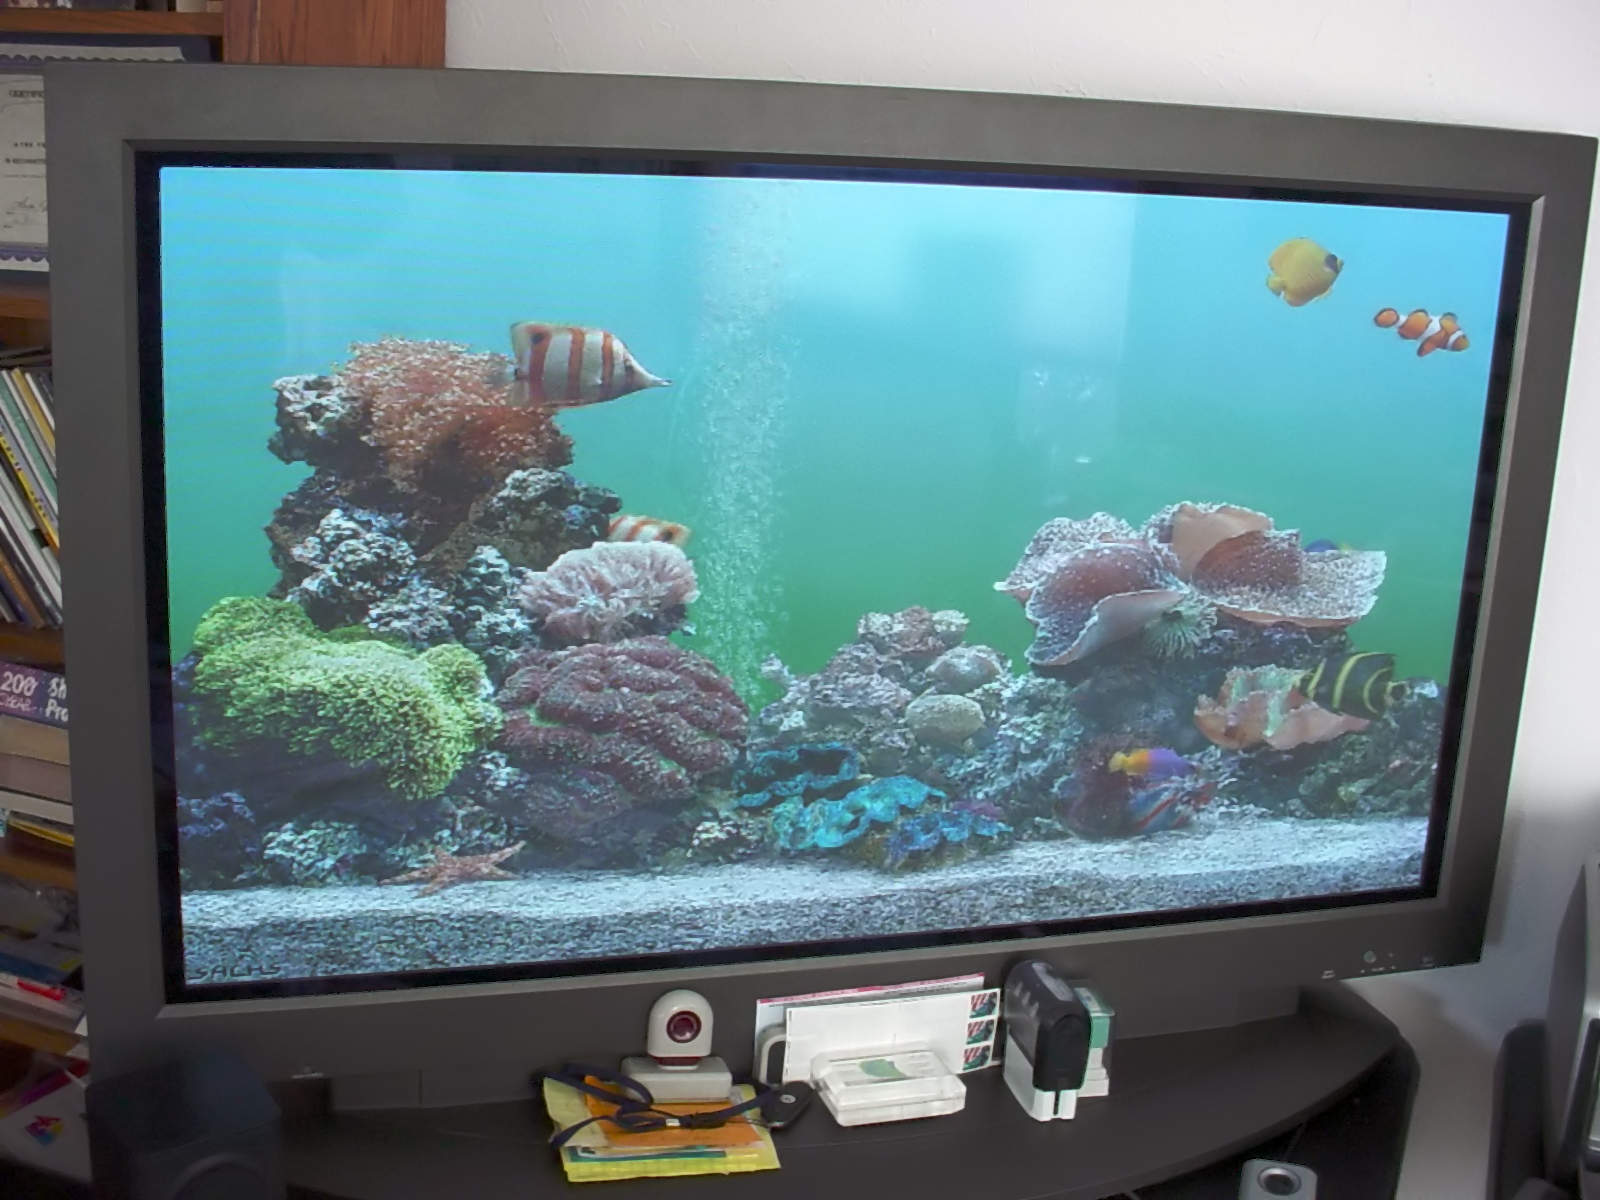
\includegraphics[width=.40\textwidth]{./figuras/plasma_display} 
  \caption{Tela de Plasma}
  \label{fig:plasma_display} 
\end{figure}

O primeiro monitor monocromático de plasma foi desenvolvido em 1964 para os computadores PLATO (PLATO Computer System), em parceria com a Universidade de Illinois em Urbana-Champaign por Donald Bitzer, H. Gene Slottow e o estudante Robert Wilson. As vantagens da aplicação de monitores de plasma em informática até meados da década de 70, eram sua robustez e por não necessitarem de buffer de dados para atualização de imagens. Com a queda de preço dos semicondutores (Lei de Moore) os CRTs dominaram o mercado até o final dos anos 90 \cite{WikipediaTelaPlasma}.\\

Em 1997, a Fujitsu introduziu o primeiro televisor de plasma com 42 polegadas no varejo. Este tinha resolução de 852 x 480 (EDTV), varredura progressiva e custava US\$14.999 à sua estréia \cite{WikipediaTelaPlasma}.\\

A tela de plasma possui algumas camadas em sua composição conforme é possível ver na figura \ref{fig:camadas_plasma}.\\

Esta tecnologia ficou muito famosa em televisores, no entanto, não foi uma tecnologia viável para dispositivos móveis pela sua tecnologia não ser tão portátil. 


%% ------------------------------------------------------------------------- %%
\section{LCD - Liquid Crystal Display}
\label{sec:lcd}

\begin{figure}[!ht]
  \centering
  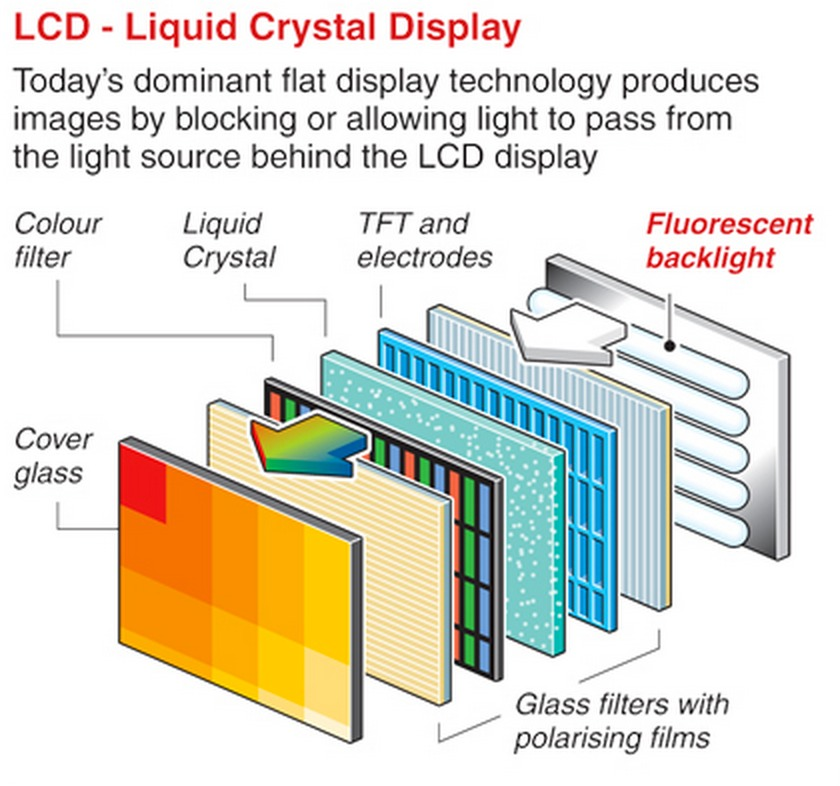
\includegraphics[width=.40\textwidth]{./figuras/camadas_lcd} 
  \caption{Camadas de uma Tela de LCD}
  \label{fig:camadas_lcd} 
\end{figure}

Um LCD consiste de um líquido polarizador da luz, eletricamente controlado, que se encontra comprimido dentro de celas entre duas lâminas transparentes polarizadoras. Os eixos polarizadores das duas lâminas estão alinhados perpendicularmente entre si. Cada cela é provida de contatos eléctricos que permitem que um campo elétrico possa ser aplicado ao líquido no interior.\\

Entre as suas principais características está a sua leveza, sua portabilidade, e sua capacidade de ser produzido em quantidades muito maiores do que os tubos de raios catódicos (CRT). Seu baixo consumo de energia elétrica lhe permite ser utilizado em equipamentos portáteis, alimentados por bateria eletrônica. É um dispositivo eletrônico-óptico modulado, composto por um determinado número de pixels, preenchidos com cristais líquidos e dispostos em frente a uma fonte de luz para produzir imagens em cores ou preto e branco \cite{WikipediaLCD}.\\

A mais antiga descoberta que levou ao desenvolvimento da tecnologia LCD foi a descoberta dos cristais líquidos, em 1888. Em 2008 as vendas mundiais de televisores com telas de LCD superaram a venda de unidades CRT. Um monitor de cristal líquido é um monitor muito leve e fino, sem partes móveis \cite{WikipediaLCD}.\\

A tecnologia LCD já é utilizada há algum tempo. Como exemplo, podemos citar consoles portáteis que começaram no Gameboy (Nintendo), relógios digitais, calculadoras, mp4, mp3, DVDs portáteis, câmeras digitais e celulares \cite{WikipediaLCD}.\\

Em 17 de Março a companhia italiana Technovision lança luXio, a maior TV LCD do mundo, com 205 polegadas, superando assim as TVs da Samsung, de 84 polegadas; da Panasonic, de 103 polegadas; da Sharp, de 108 polegadas; e da veterana Panasonic com 150 polegadas \cite{WikipediaLCD}. \\

A tela de LCD possui algumas camadas em sua composição conforme é possível ver na figura \ref{fig:camadas_lcd}.\\


%% ------------------------------------------------------------------------- %%
\section{LED - Light Emitting Diode}
\label{sec:led}

\begin{figure}[!ht]
  \centering
  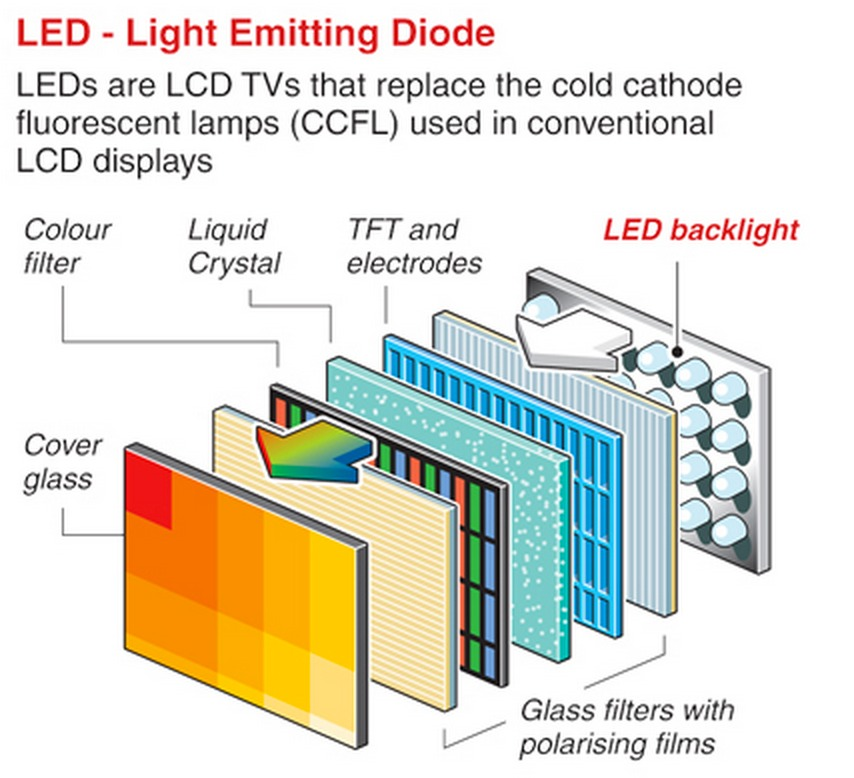
\includegraphics[width=.40\textwidth]{./figuras/camadas_led} 
  \caption{Camadas de uma Tela de LED}
  \label{fig:camadas_led} 
\end{figure}

O LED é propriamente dito um Diodo Emissor de Luz, uma espécie de componente eletrônico semicondutor que tem a capacidade de transformar energia elétrica em luz. Já as lâmpadas comuns utilizam radiação ultravioleta com descarga de gases, como no caso das lâmpadas fluorescentes usadas nas tecnologias Plasma e LCD. \\

O princípio do LED não foi uma invenção recente. Segundo dados pesquisados e divulgados pelo projeto Laboratório de Iluminação da Unicamp, o LED foi desenvolvido ainda que em fase experimental e rudimentar no ano de 1963 por Nick Holonyac. Seu funcionamento era apenas pela luz vermelha e com baixa luminosidade, atingindo apenas 1 mcd. Em 1960 obteve o LED amarelo e apenas em 1975 que surgiu a luz verde. Isso representa que o LED de hoje é muito mais avançado, mas a descoberta de Holonyac foi o processo inicial para a invenção da tecnologia LED.\\

Foi no início dos anos 90 que houve a verdadeira revolução do LED e a possibilidade de aplicá-lo no setor automotivo, por exemplo. Com o surgimento da tecnologia INGan, foi possível obter-se LEDs com comprimento de ondas menores, nas cores azul, verde e ciano, tecnologia esta que propiciou a obtenção do LED branco, e consequentemente, todos os espectros de cores.\\

Mas foi com o surgimento da tecnologia Luxeon que foi possível ter fluxo luminoso de 30 lumens e com um ângulo de emissão de 110 graus, e não mais as antigas ondas de intensidades, conseguindo assim maior rendimento e avanço tecnológico no assunto.\\

Por muitos anos a tecnologia LED foi utilizada como sinais de indicação de estado para aparelhos eletrônicos, como rádio, televisão e outros aparelhos. É a típica luz vermelha que indica quando o aparelho se encontra ligado ou desligado. Hoje, o LED é muito aplicado em automóveis, destacando o veículo e proporcionando melhor luminosidade com baixo consumo de energia. Também é utilizado em Painéis de Led. Estes aparelhos são aplicados para cenografia, shows, feiras e eventos, exibição de propagandas (principalmente por meio de Painel de Led Outdoor), estúdios de TV, e muitas outras ocasiões.\\

O Painel de Led é formado por placas compostas por pequenas lâmpadas de luzes RGB (Red, Green, Blue) formando assim os pixels, responsáveis pela composição das imagens. As camadas que compoem a tela LED é possível ver na figura \ref{fig:camadas_led}.\\




















